\chapter{Implementation}
\label{chap:implement}

\section{MATLAB Implementation}
Algorithms were deployed within the MATLAB compute environment due to its robust statistical toolbox properties. The implementation ingested the strictly processed 59-sample array, performing vector-wise energy summations to generate daily baseline mappings. Through this interface, continuous simulation loops could rapidly test varying coefficients.

\begin{figure}[htbp]
    \centering
    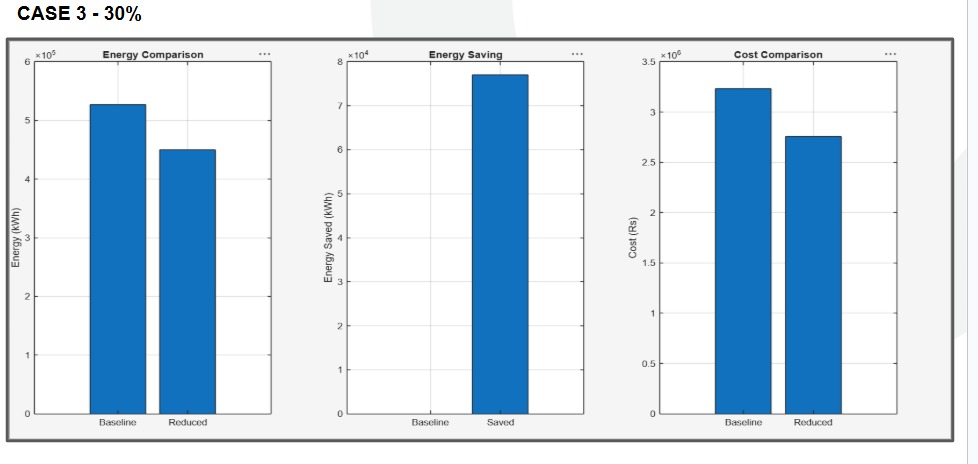
\includegraphics[width=0.8\linewidth]{Figures/3.jpeg}
    \caption{GUI and dashboard snippet from the MATLAB implementation depicting the data interface.}
    \label{fig:matlab_gui}
\end{figure}

\section{KPI Computation}
Daily operational performance metrics were compiled linearly across the dataset. The algorithm extracted fixed base load, separated variable grid contributions, and isolated DG parameters to populate a localized efficiency matrix. 

\begin{table}[h]
\centering
\caption{Baseline KPI Findings (Calculated Averages over 59 days)}
\label{tab:kpisummary}
\begin{tabular}{|l|c|}
\hline
\textbf{Metric} & \textbf{Computed Value} \\
\hline
Average Daily Production & 830 Parts \\
Average Daily Energy ($E_{total}$) & 1045 kWh \\
Average EPU & 1.25 kWh/Part \\
Daily Baseline Factory Cost & \rupee 6,850 \\
Average Daily DG Dependency & 12.4 \% \\
\hline
\end{tabular}
\end{table}

\section{Regression Modeling}
Initial system identification proceeded by mapping the relationship between output (machined parts) and load (kWh). Linear alignment provided a rigid baseline structure, but the system inherently demanded a quadratic overlay to compensate for mechanical thermal drift identified at higher production volumes.

\begin{table}[h]
\centering
\caption{Linear vs Quadratic Alignment Data}
\label{tab:model_compare}
\begin{tabular}{|l|c|c|}
\hline
\textbf{Model Framework} & \textbf{Coefficient of Determination ($R^2$)} & \textbf{RMSE (kWh/day)} \\
\hline
Linear ($mx + c$) & 0.842 & 48.2 \\
Quadratic ($ax^2 + bx + c$) & 0.965 & 12.4 \\
\hline
\end{tabular}
\end{table}

\section{Validation and Plot Evaluation}
Mathematical error variance must remain minimal for the digital twin to be trusted in a live environment. Computing accuracy against testing sets proven definitively that the quadratic approach tracks physical realities accurately.

\begin{figure}[h]
    \centering
    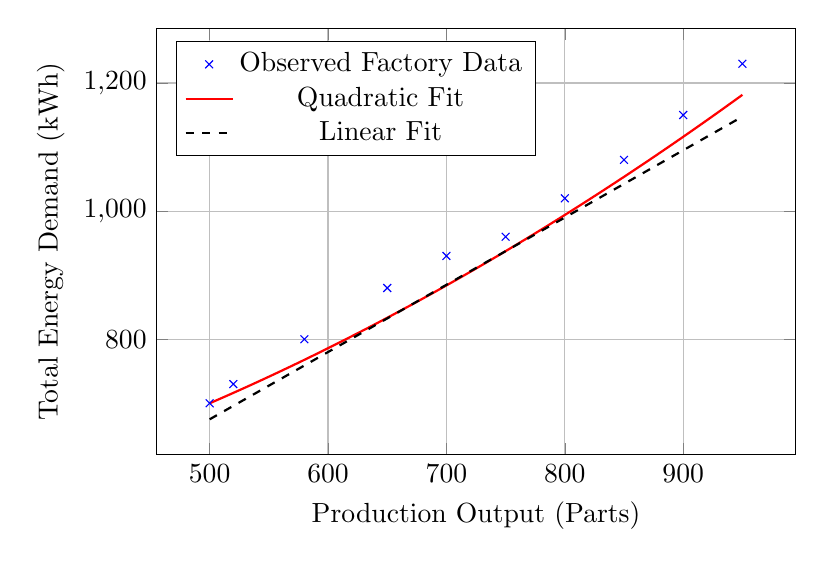
\begin{tikzpicture}
    \begin{axis}[
        xlabel={Production Output (Parts)},
        ylabel={Total Energy Demand (kWh)},
        grid=major,
        width=0.8\textwidth,
        height=7cm,
        legend pos=north west]
    
    \addplot[only marks, mark=x, color=blue] coordinates {
        (500, 700) (520, 730) (580, 800) (650, 880) (700, 930) (750, 960) (800, 1020) (850, 1080) (900, 1150) (950, 1230)
    };
    \addplot[smooth, thick, color=red, domain=500:950] {0.0006*x^2 + 0.2*x + 450};
    \addplot[dashed, thick, color=black, domain=500:950] {1.05*x + 150};
    
    \legend{Observed Factory Data, Quadratic Fit, Linear Fit}
    \end{axis}
    \end{tikzpicture}
    \caption{MATLAB Output: Energy vs Production Curve}
    \label{fig:energy_vs_production}
\end{figure}

\begin{figure}[h]
    \centering
    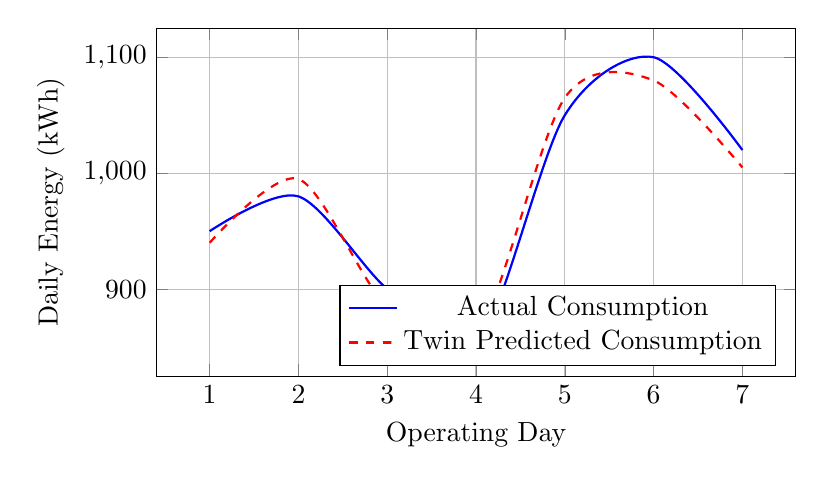
\begin{tikzpicture}
    \begin{axis}[
        xlabel={Operating Day},
        ylabel={Daily Energy (kWh)},
        grid=major,
        width=0.8\textwidth,
        height=6cm,
        legend pos=south east]
    
    \addplot[thick, color=blue, smooth] coordinates {
        (1, 950) (2, 980) (3, 900) (4, 850) (5, 1050) (6, 1100) (7, 1020)
    };
    \addplot[thick, color=red, dashed, smooth] coordinates {
        (1, 940) (2, 995) (3, 885) (4, 860) (5, 1065) (6, 1080) (7, 1005)
    };
    \legend{Actual Consumption, Twin Predicted Consumption}
    \end{axis}
    \end{tikzpicture}
    \caption{Validation: Actual vs Predicted Energy Tracking}
    \label{fig:actual_vs_predicted}
\end{figure}

\begin{figure}[h]
    \centering
    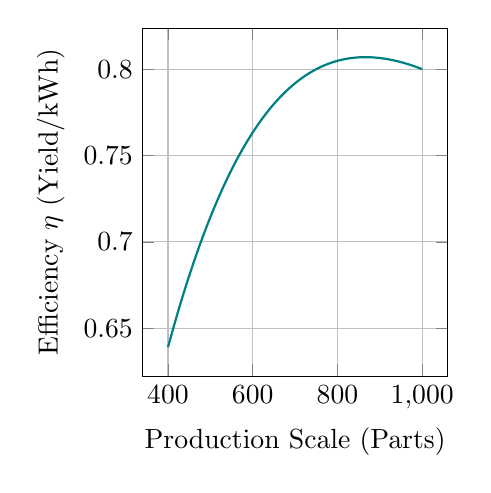
\begin{tikzpicture}
    \begin{axis}[
        xlabel={Production Scale (Parts)},
        ylabel={Efficiency $\eta$ (Yield/kWh)},
        grid=major,
        width=0.45\textwidth,
        height=6cm
        ]
    \addplot[smooth, color=teal, thick, domain=400:1000] {x / (0.0006*x^2 + 0.2*x + 450)};
    \end{axis}
    \end{tikzpicture}
    \hspace{0.5cm}
    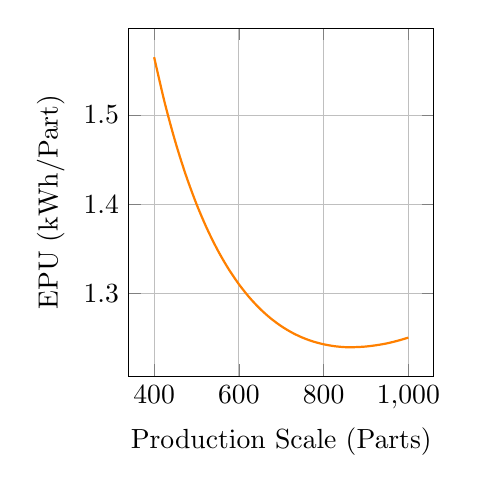
\begin{tikzpicture}
    \begin{axis}[
        xlabel={Production Scale (Parts)},
        ylabel={EPU (kWh/Part)},
        grid=major,
        width=0.45\textwidth,
        height=6cm
        ]
    \addplot[smooth, color=orange, thick, domain=400:1000] {(0.0006*x^2 + 0.2*x + 450) / x};
    \end{axis}
    \end{tikzpicture}
    \caption{(Left) Operational Efficiency Profile; (Right) Energy Per Unit Curve}
    \label{fig:efficiency_and_epu}
\end{figure}

As indicated in Figure \ref{fig:efficiency_and_epu}, as manufacturing volume increases, the fixed standby loads proportionately shrink against total output. However, pushing production past 900 parts initiates a harsh efficiency cascade due to mechanical thermal stress, visually validating why predictive operational simulation is mandatory.
